% Preamble
%\documentclass[xetex,mathserif,serif]{beamer}
\documentclass{beamer}

% Packages
\usepackage[spanish]{babel}
\selectlanguage{spanish}
\usepackage[utf8]{inputenc} % For spanish (and international) letters like acents.
\usepackage{hyperref} % To create hyperlinks within the document.
\usepackage{graphicx} % To include graphics (pictures, images)
\usepackage{float} % For the use of the parameter "H" in command "\begin{figure}[H]" (i.e. exact position of image in text)
\usepackage{verbatim} % For long comments
\usepackage{tikz} % For include Dia diagrams in .tex format

\graphicspath{{../Diagramas/}} % Path of the folder containing the images

\title{Del código a la catalogación}
\subtitle{El sistema web para la catalogación y acceso de la colección de documentales del LAIS}
\author{Rodrigo Colín Rivera, Sergio Amaro Rosas}
\institute
{
  Laboratorio Audiovisual de Investigación Social\\
  Instituto de Investigaciones Dr. José María Luis Mora
}
\date{\today}
\subject{Catalogación de Colección de Documentales}

\begin{comment}
\AtBeginSection[]
{
  \begin{frame}
    \frametitle{Tabla de contenidos}
    \tableofcontents[currentsection]
  \end{frame}
}
\AtBeginSubsection[]
{
  \begin{frame}
    \frametitle{Tabla de contenidos}
    \tableofcontents[currentsection,currentsubsection]
  \end{frame}
}
\end{comment}

% Style and theme
\usetheme{PaloAlto}
%\usecolortheme{orchid} %crane,dolphin,lily

% Document environment
\begin{document}

\frame{\titlepage} % Página inicial

\section{Colección documental del LAIS}
\begin{frame}
	\frametitle{El LAIS}
	\framesubtitle{Colección documental del LAIS}
	
	El LAIS ha construido un acervo documental que se origina en 1993, año en que inicia la producción de su primer documental: \textit{Un pueblo en la memoria}.

	Para el LAIS es una tarea prioritaria el resguardo y documentación de materiales audiovisuales para quienes recurrimos a ellos con fines de investigación.
	
\end{frame}

\section{Catalogación}
\begin{frame}
	\frametitle{Catalogación}
	\framesubtitle{Acerca de ISAD(G)}
	
	¿Para qué catalogar?: Para preservar y \textbf{utilizar}.
	
	Por lo tanto se emplea la norma \textbf{ISAD(G)} (\textit{General International Standard Archival Description}) como base para la catalogación, ya que es el estándar para registrar documentos de archivo.
\end{frame}

\begin{frame}
	\frametitle{Catalogación}
	\framesubtitle{Colección de materiales audiovisuales del LAIS}
	
	La colección integra tres series:
	\begin{enumerate}
		\item Documentales en video
		\item Registros en video
		\item Material de archivo
	\end{enumerate}
	
	El énfasis del sitio está dado en la serie de \textbf{Documentales en video}. Constituida por \textbf{cine documental} recopilado desde los antecedentes del LAIS en diversos videoforos y cursos relacionados desde 1995.
	
\end{frame}

\section{Manual de Catalogación}
\begin{frame}
	\frametitle{Manual de Catalogación}
	\framesubtitle{Para el acervo documental en video del LAIS}
	
	Para el caso particular de la colección de documentales en video del LAIS, la norma ISAD(G) es adaptada y el resultado es el ``\textbf{Manual de Catalogación para Documentales en Video del LAIS}'' que contempla las siguientes áreas de descripción:
	
	\begin{enumerate}
		\item Identificación
		\item Contexto
		\item Contenido y estructura
		\item Condiciones de acceso y uso
		\item Documentación asociada
		\item Notas
		\item Control de la descripción
	\end{enumerate}
\end{frame}

\section{Situación y propuesta}
\begin{frame}
	\frametitle{Situación y Propuesta}
	\framesubtitle{Para poner en acceso la ficha de los documentales}
	
	Las fichas de documentación se tenían registradas en \textbf{hojas de cálculo} de Excel, de manera que la propuesta fue la siguiente:
	
	Hacer un \textbf{sistema} que administre y ponga en \textbf{acceso} estas fichas documentales; para lo cual se requiere crear una base de datos y una interfaz visual con la que los usuarios (los integrantes del LAIS y las personas interesadas en la ficha documental) puedan consultar dicha información.
\end{frame}

\section{Sistema}
\begin{frame}
	\frametitle{El sistema}
	\framesubtitle{Esquema general}
	\begin{figure}[H]
		\centering
		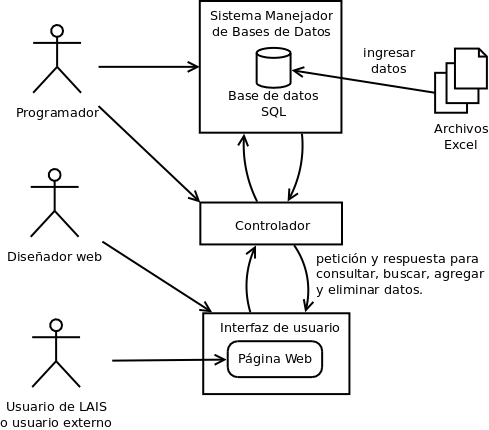
\includegraphics[width=0.7\textwidth]{EsquemaGeneral.png}
		\caption{Esquema general del sistema (aplicación web) para la catalogación y acceso de la colección de documentales del LAIS}
		\label{fig:esquema_general}
	\end{figure}
\end{frame}

\section{Requisitos}
\begin{frame}
	\frametitle{Requisitos a cumplir}
	
	\begin{itemize}
		\item Crear y poblar la base de datos con la información existente.
		\item Permitir agregar, modificar y eliminar fichas de documentación.
		\item Crear un sitio web (interfaz) eficiente y simple de usar.
		\item Control de quién puede realizar cambios en el sistema.
		\item Realizar búsquedas.
	\end{itemize}
\end{frame}

\section{Demostración}
\begin{frame}
	\frametitle{Demostración}
	\framesubtitle{Primera versión del sistema}
	
	\begin{figure}[H]
		\centering
		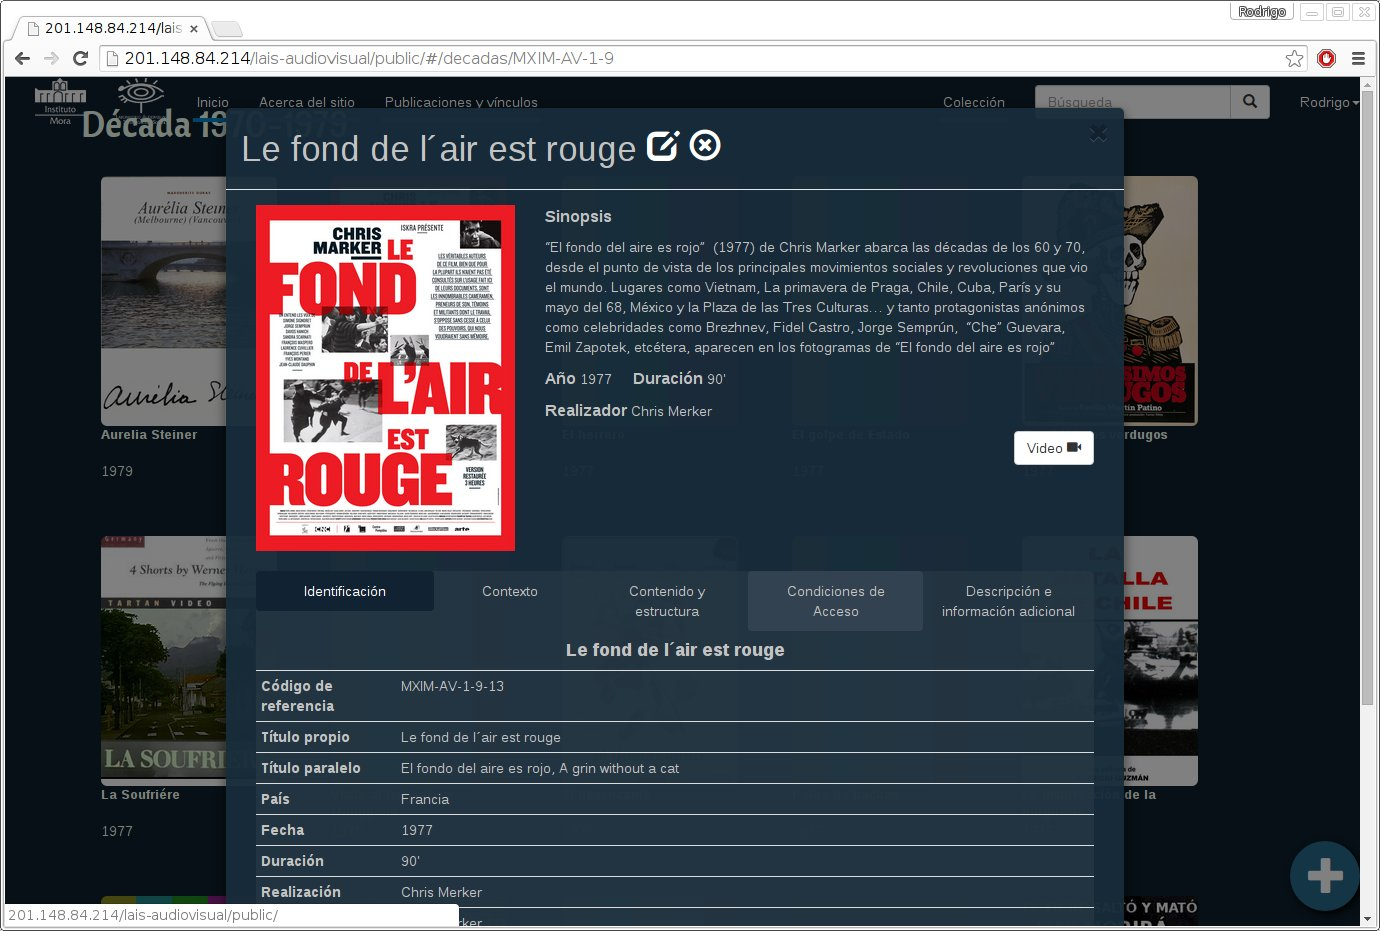
\includegraphics[width=0.7\textwidth]{Sistema01.jpg}
		\caption{Captura de pantalla del \href{http://201.148.84.214/lais-audiovisual/public}{sistema}, muestra la ficha de un documental. (\url{lais-interno.mora.edu.mx/lais-audiovisual/public/})}
		\label{fig:sistema01}
	\end{figure}
\end{frame}

\section{Diseño}
\begin{frame}
	\frametitle{Acerca del diseño}
	\framesubtitle{Elementos visuales y de interacción con el usuario}
	
	Un buen diseño de los elementos visuales ayuda a que los usuarios sepan usar el sistema de mejor manera. Por ejemplo:
	
	\begin{itemize}
		\item Énfasis en lo visual (portadas).
		\item Navegación simple y rápida del contenido.
		\item Diseño responsivo.
	\end{itemize}
\end{frame}

\section{Conclusión}
\begin{frame}
	\frametitle{Conclusiones}
	\begin{itemize}
		\item Mediante este sistema, incentivar la \textbf{consulta} de la ficha y los contenidos de los materiales audiovisuales para todas las personas interesadas.
		\item Permitió una revisión y \textbf{reflexión} acerca de la forma de documentar.
		\item El uso de \textbf{software libre} para dar soluciones a problemas de reguardo y documentación de materiales audiovisual.
		\item La escalabilidad y futuro \textbf{desarrollo} del sistema.
	\end{itemize}
\end{frame}

\begin{frame}
	\begin{center}
		GRACIAS POR SU TIEMPO.
		
		%logo del LAIS
		%
\includegraphics{scientistapprovedfutura.png}
	\end{center}
\end{frame}

\end{document}